\pagestyle{empty}

\def\layersep{2.5cm}
\begin{center}
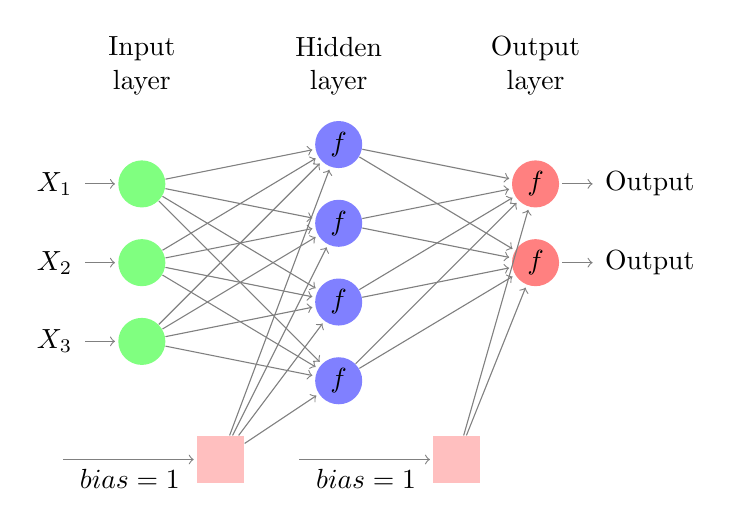
\begin{tikzpicture}[shorten >=1pt,->,draw=black!50, node distance=\layersep]
    \tikzstyle{every pin edge}=[<-,shorten <=1pt]
    \tikzstyle{neuron}=[circle,fill=black!25,minimum size=17pt,inner sep=0pt]
    \tikzstyle{bias}=[rectangle,fill=red!25,minimum size=17pt,inner sep=0pt]
    \tikzstyle{input neuron}=[neuron, fill=green!50];
    \tikzstyle{output neuron}=[neuron, fill=red!50];
    \tikzstyle{hidden neuron}=[neuron, fill=blue!50];
    \tikzstyle{annot} = [text width=4em, text centered]

    % Draw the input layer nodes
    \foreach \name / \y in {1,...,3}
    % This is the same as writing \foreach \name / \y in {1/1,2/2,3/3,4/4}
        \node[input neuron, pin=left:$X_{\y}$] (I-\name) at (0,-\y) {};

    % Draw the hidden layer nodes
    \foreach \name / \y in {1,...,4}
        \path[yshift=0.5cm]
            node[hidden neuron] (H-\name) at (\layersep,-\y cm) {$f$};

    % Draw the output layer node
    \foreach \name / \y in {1,2}
        \node[output neuron, pin={[pin edge={->}]right:Output},right of=H-2] (O-\name) at (2.5,-\y) {$f$};

    % Connect every node in the input layer with every node in the
    % hidden layer.
    \foreach \source in {1,...,3}
        \foreach \dest in {1,...,4}
            \path (I-\source) edge (H-\dest);

    % Connect every node in the hidden layer with the output layer
    \foreach \source in {1,...,4}
        \path (H-\source) edge (O-1);
    \foreach \source in {1,...,4}
        \path (H-\source) edge (O-2);

    % Annotate the layers
    \node[annot,above of=H-1, node distance=1cm] (hl) {Hidden layer};
    \node[annot,left of=hl] {Input layer};
    \node[annot,right of=hl] {Output layer};

    %new bias diagram
    \node[bias] (B-1) at (1,-4.5) {};
    \node[bias] (B-2) at (4,-4.5) {};

    \foreach \hidden in {1,...,4}
        \path (B-1) edge (H-\hidden);
    \foreach \hidden in {1,2}
        \path (B-2) edge (O-\hidden);

    \path[->] (-1,-4.5) edge node [below] {$bias=1$} (B-1);
    \path[->] (2,-4.5) edge node [below] {$bias=1$} (B-2);

\end{tikzpicture}
\end{center}
